\begin{frame}[allowframebreaks]{Improving ViT: Distillation}
    \begin{itemize}
        \item Data-efficient ViT \& DeiT approach uses \textit{knowledge distillation} from CNN teacher models to improve data efficiency and convergence.
        \item Benefits: better performance with fewer data and better optimization stability.
    \end{itemize}
    \framebreak
    \begin{figure}
        \centering
        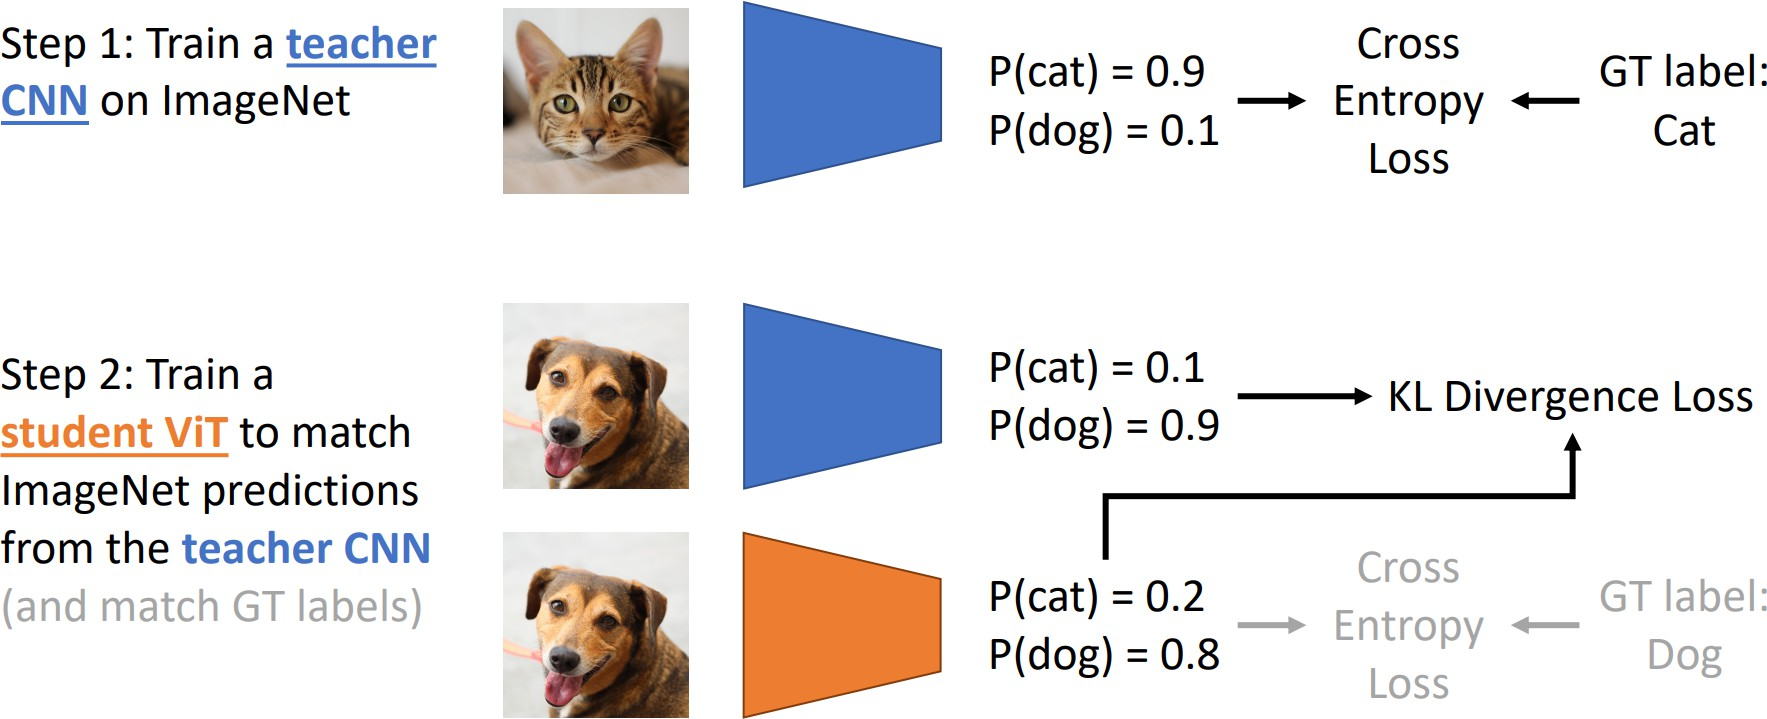
\includegraphics[width=\linewidth,height=0.9\textheight,keepaspectratio]{images/vit/slide_65_1_img.jpg}
    \end{figure}

    \framebreak

    \begin{figure}
        \centering
        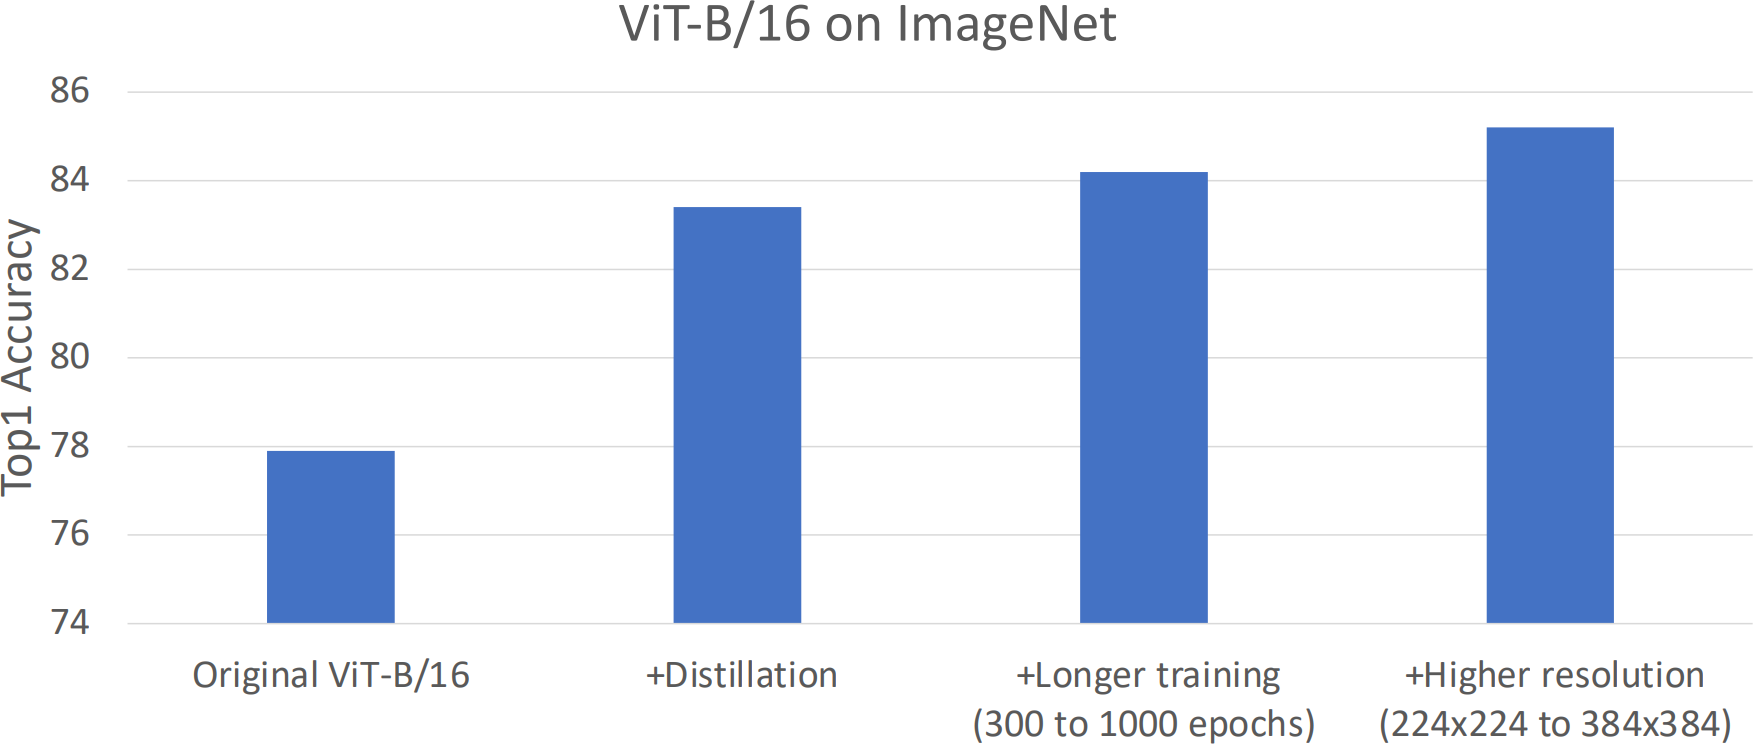
\includegraphics[width=\linewidth,height=\textheight,keepaspectratio]{images/vit/slide_66_1_img.png}
        \footnote{Touvrom et al, “Training data-efficient image transformers distillation through attention”, ICML 2021}
    \end{figure}
\end{frame}